\documentclass{iopart}

\usepackage{url}
\usepackage{amsbsy}
\usepackage{graphicx}

\newcommand{\eqref}[1]{{(\ref{#1})}}
 
\begin{document}

\title{A report on the second Mock LISA Data Challenge} 

\author{The \emph{Mock LISA Data Challenge Task Force}:
Stanislav Babak$^1$,
John G. Baker$^2$,
Matthew J. Benacquista$^3$,
Neil J. Cornish$^4$,
Jeff Crowder$^5$,
Curt Cutler$^5$,
Shane L. Larson$^6$,
Tyson B. Littenberg$^4$,
Edward K. Porter$^1$,
Michele Vallisneri$^5$,
Alberto Vecchio$^{7,8}$ and \emph{the Challenge-2 participants}:
Gerard Auger$^9$, Leor Barack$^{10}$, Arkadiusz Blaut$^{11}$, Ed Bloomer$^{12}$, Duncan A. Brown$^{13,14}$, Nelson Christensen$^{15}$, James Clark$^{12}$, Stephen Fairhurst$^{13,14}$, Jonathan R. Gair$^{16}$, Hubert Halloin$^9$, Martin Hendry$^{12}$, Arturo Jimenez$^3$, Andrzej Kr\'olak$^{11}$, Ilya Mandel$^{14}$, Chris Messenger$^{12}$, Renate Meyer$^{17}$, Soumya Mohanty$^3$, Rajesh Nayak$^3$, Antoine Petiteau$^9$, Matt Pitkin$^{12}$, Eric Plagnol$^9$, Reinhard Prix$^1$, Emma L. Robinson$^7$, Christian Roever$^{17}$, Pavlin Savov$^{14}$, Alexander Stroeer$^{7,8}$, Jennifer Toher$^{12}$, John Veitch$^7$, Jean--Yves Vinet$^{18}$, Linqing Wen$^1$, John T. Whelan$^1$, Graham Woan$^{12}$}

\address{$^1$ Max-Planck-Institut f\"ur Gravitationsphysik (Albert-Einstein-Institut), Am M\"uhlenberg 1, D-14476 Golm bei Potsdam, Germany}
\address{$^2$ Gravitational Astrophysics Laboratory, NASA Goddard Space Flight Center, 8800 Greenbelt Rd., Greenbelt, MD 20771, USA}
\address{$^3$ Center for Gravitational Wave Astronomy, University of Texas at Brownsville, Brownsville, TX 78520, USA}
\address{$^4$ Department of Physics, Montana State University, Bozeman, MT 59717, USA}
\address{$^5$ Jet Propulsion Laboratory, California Institute of Technology, Pasadena, CA 91109, USA}
\address{$^6$ Department of Physics, Weber State University, 2508 University Circle, Ogden, UT 84408, USA}
\address{$^7$ School of Physics and Astronomy, University of Birmingham, Edgbaston, Birmingham B152TT, UK}
\address{$^8$ Department of Physics and Astronomy, Northwestern University, Evanston, IL, USA}
\address{$^9$ APC, UMR 7164, University Paris 7 Denis Diderot, 10, rue Alice 
Domon et Leonie Duquet, 75025 Paris Cedex 13, France}
\address{$^{10}$ School of Mathematics, University of Southampton, Southampton, SO171BJ, UK}
\address{$^{11}$ Institute of Mathematics, Polish Academy of Sciences, Warsaw, Poland}
\address{$^{12}$ Department of Physics and Astronomy, University of Glasgow, Glasgow, UK}
\address{$^{13}$ LIGO Laboratory, California Institute of Technology, Pasadena, CA 91125}
\address{$^{14}$ Theoretical Astrophysics, California Institute of Technology, Pasadena, CA 
91125}
\address{$^{15}$ Physics and Astronomy, Carleton College, Northfield, MN, USA}
\address{$^{16}$ Institute of Astronomy, University of Cambridge, Cambridge, CB30HA, UK}
\address{$^{17}$ Department of Statistics, The University of Auckland, Auckland, New Zealand}
\address{$^{18}$ ARTEMIS, Observatoire de la Cote d'Azur-C.N.R.S., 06304 Nice, France} 

\ead{Michele.Vallisneri@jpl.nasa.gov}

\begin{abstract}
The Mock LISA Data Challenges are a program to demonstrate LISA data-analysis capabilities and to encourage their development. Each round of challenges consists of several data sets containing simulated instrument noise and gravitational-wave sources of undisclosed parameters. Participants are asked to analyze the data sets and report the maximum information about source parameters. The  
challenges are being released in rounds of increasing complexity and realism, and so far they have already demonstrated the recovery of model signals from supermassive black-hole binaries, from ~ 20,000 overlapping Galactic white-dwarf binaries, and from the extreme--mass-ratio inspirals of compact objects into central galactic black holes. We discuss the results and details of the program.
\end{abstract}

\vspace{-12pt}
\pacs{04.80.Nn, 95.55.Ym}

% \maketitle

\section{Introduction}

The Laser Interferometer Space Antenna (LISA), a NASA/ESA space mission to detect gravitational waves in the $10^{-5}$--$10^{-1}$ Hz range \cite{lisa}, will produce time series consisting of the superposition of the gravitational waves (GWs) from all sources within range, typically thousands. Some of the gravitational signals (such as those from extreme--mass-ratio inspirals, or EMRIs) are very complex functions of the physical parameters of the sources; others (such as those from Galactic white-dwarf binaries) are simpler, but their resolution will be confused by the presence of many similar signals, overlapping in frequency space. Thus, data analysis is integral to the LISA measurement concept, because no physical source can be identified without first carefully teasing out its individual voice from the noisy party of each data set. Understanding data analysis is therefore important to demonstrate that LISA can meet its science requirements and to translate them into decisions about instrument design.

The idea of the Mock LISA Data Challenges (MLDCs) arose in late 2005 from this realization. The MLDCs have the purpose of encouraging and tracking progress in LISA data-analysis development, and (as a useful byproduct) of prototyping a computational infrastructure for LISA data analysis, which includes common data formats, standard models of the LISA orbits, noises and measurement, descriptions of the waveforms and populations of targeted GW sources, and so on.
The MLDCs are a coordinated (but voluntary) effort in the GW community, whereby a task force chartered by the LISA International Science Team periodically issues a number of datasets with 
synthetic noise and GW signals from sources of undisclosed parameters; challenge participants return detection candidates and parameter estimates, together with descriptions of their search methods. These results are then compiled and compared to the previously secret challenge ``key''.
%
\begin{figure}
\caption{Mock LISA Data Challenges timeline.\label{fig:timeline}}
\end{figure}

Figure \ref{fig:timeline} shows the timeline and progression of MLDCs. Challenge 1 (see Refs.\ YYY and ZZZ) tackled the detection and parameter characterization of \emph{verification binaries} (Galactic binaries of known frequency and position); of loud unknown Galactic binaries, either alone or in small, moderately interfering groups; and of relatively loud inspirals of supermassive--black-hole (MBH)  binaries. All sources were represented by moderately idealized waveforms, and they were staged on instrument noise alone. Altogether, Challenge 1 successfully demonstrated the detection of all three source classes. Ten research collaborations participated, adopting a variety of methods (template-bank, stochastic and genetic matched filtering; time--frequency; tomography; Hilbert transform); despite the short timescale, all challenges were ``solved'' by at least one group, although some searches locked on strong secondary maxima of parameter probabilities. More important, Challenge 1 helped set the playing field and the computational tools for the more realistic Challenge 2.

Challenge 2 raised the bar by proposing a data set (2.1) containing a full population of Galactic binary systems (about 26 million sources); a data set (2.2) containing a different realization of this Galaxy, plus 4--6 MBH binary inspirals with single-interferometer signal-to-noise ratios (SNRs) between 10 and 2000 and different coalescence times, and 5 EMRIs with SNRs between 30 and 100; and five data sets (denoted 1.3.1--5, since they were actually released at the time of Challenge 1) of a single EMRI over instrument noise alone. See Ref.\ WWW for more details about the signal models and the exact content of the data sets. Thirteen collaborations participated (comprising all the researchers listed as participants in the byline, and most task force members), submitting a total of 22 entries. Altogether, Challenge 2 successfully demonstrated the identification of $\sim 20,000$ Galactic binaries, the accurate parameter estimation of MBH inspirals, and the positive detection of EMRIs. In the rest of this paper, we describe some Challenge-2 highlights. The full set of responses, together with write-ups by all participating groups, can be found at the URL XXX; some groups are also contributing proceedings from this conference to JPCS (Ref.\ YYY).

\section{Data sets 2.1 and 2.2: The Galaxy}

Five groups submitted Galactic-binary catalogs for the 2.1 and 2.2 data sets:
%
\begin{description}
\item[GLIG] A collaboration of research groups at institutions in the UK, United States and New Zealand developed a Reversible-Jump Markov Chain Monte Carlo (MCMC) code that can sample models with different numbers of sources; for lack of time, however, they only submitted parameter sets for the verification binaries.
\item[IMPAN] Kr\'olak and Blaut used $\mathcal{F}$-statistic, template-bank--based matched filtering \cite{JKS98,KTV04}, and submitted parameters for 404 sources in data set 2.1.
\item[MTJPL] The Montana State--JPL collaboration used an MCMC code that ran separately for overlapping frequency bands and for different hypotesized numbers of sources; model comparison was then used to choose the most probable number of sources in each band. The collaboration submitted parameter sets for 19,324 source in data set 2.1, and 18,461 in data set 2.2.
\item[PrixWhelanAEI] Prix and Whelan used $\mathcal{F}$-statistic, template-bank--based matched filtering in a hierarchical scheme that enforced trigger coincidence between noise-orthogonal TDI observables. They submitted parameter sets for 1777 sources in data set 2.1, and 1737 sources in data set 2.2.
\item[UTB] Nayak, Jimenez, and Mohanty used a tomographic reconstruction technique, and submitted parameters for 3862 sources in data set 2.1.
\end{description}
%
Evaluating the performance of these searches brings up a problem of principle: the performance metric that makes the most physical sense would be a statement about how many of the true sources were recovered, and with what parameter errors. For this, however, the reported sources must first be matched one-to-one with the true sources, a nontrivial operation because of the very nature of confusion noise (consider for instance the phenomena of \emph{source blending}, where multiple true sources end up being represented by a single search template, and of \emph{template blending}, where multiple templates end up representing a single strong source).
%
\begin{figure}
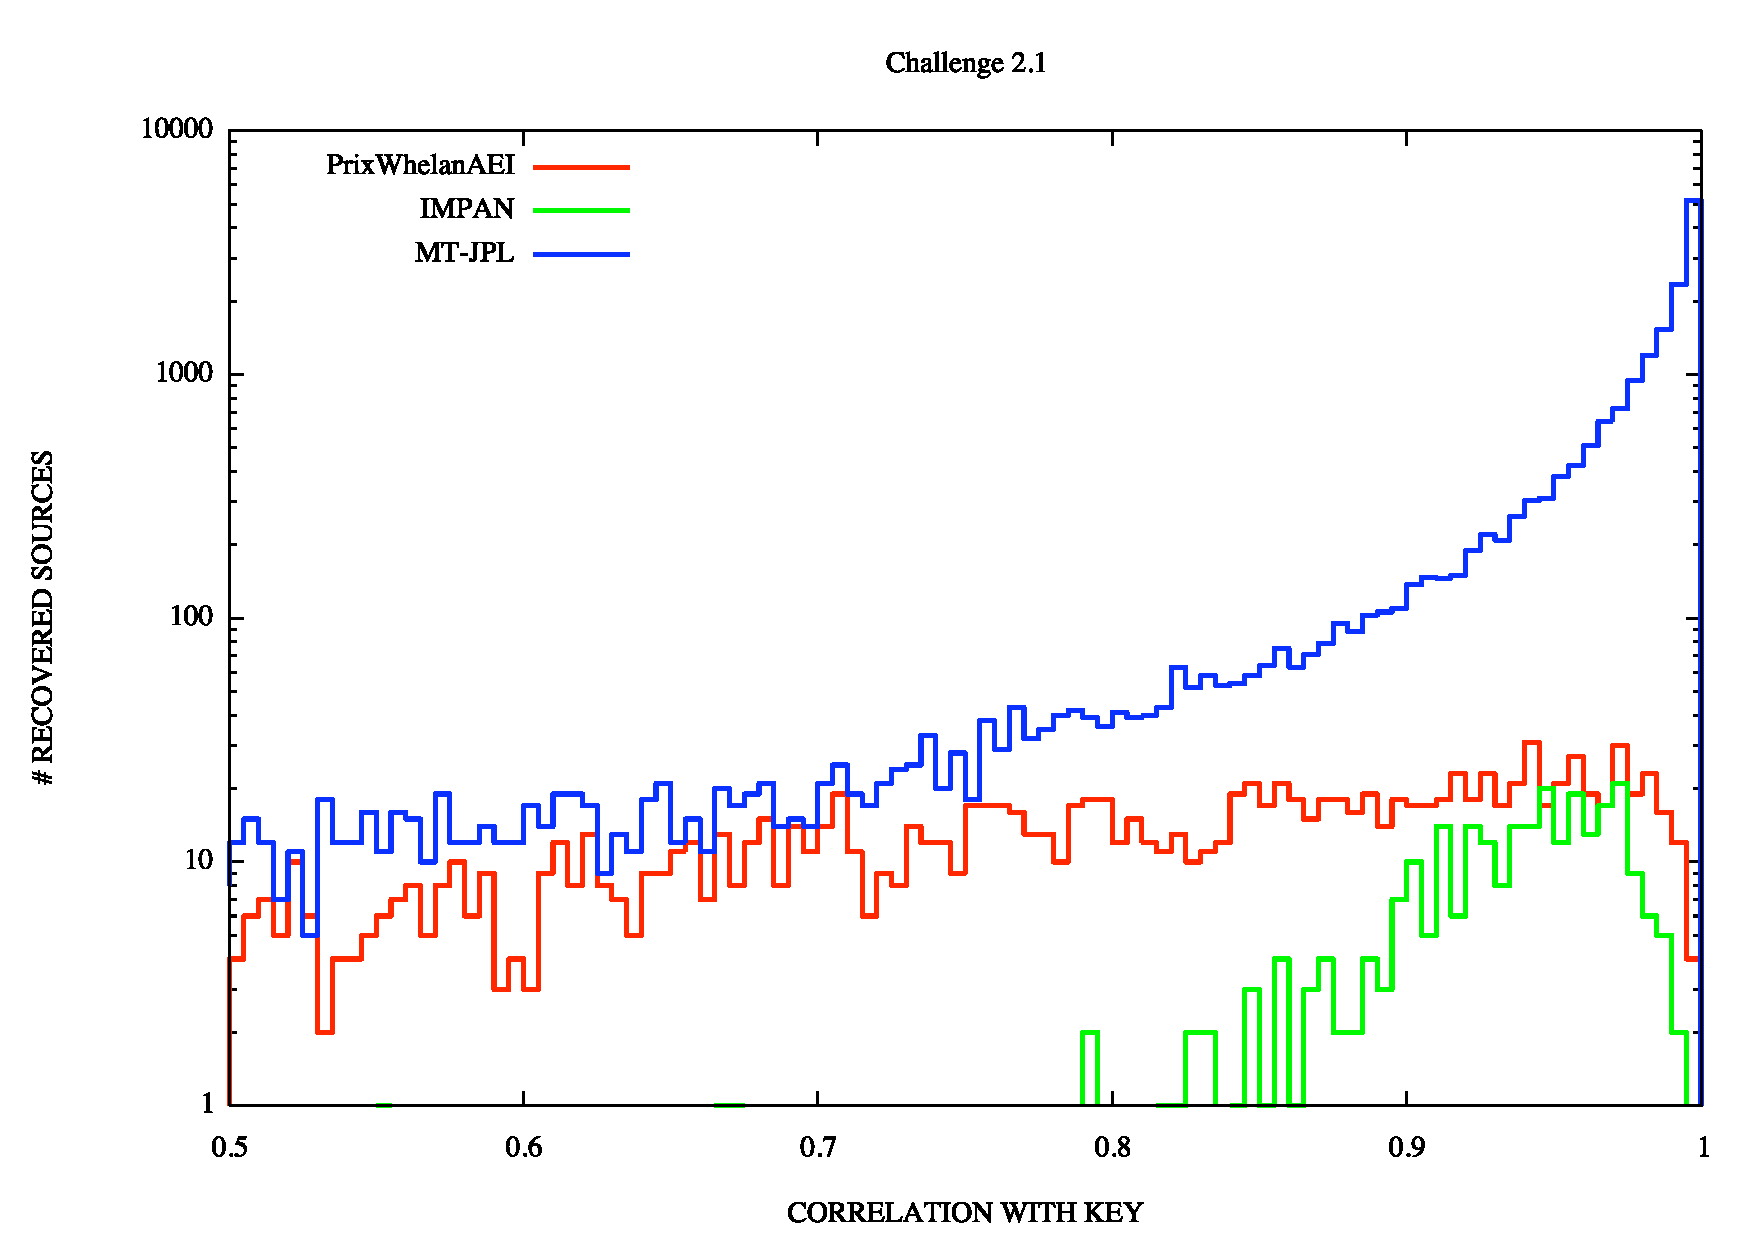
\includegraphics[width=0.5\textwidth]{correlation}
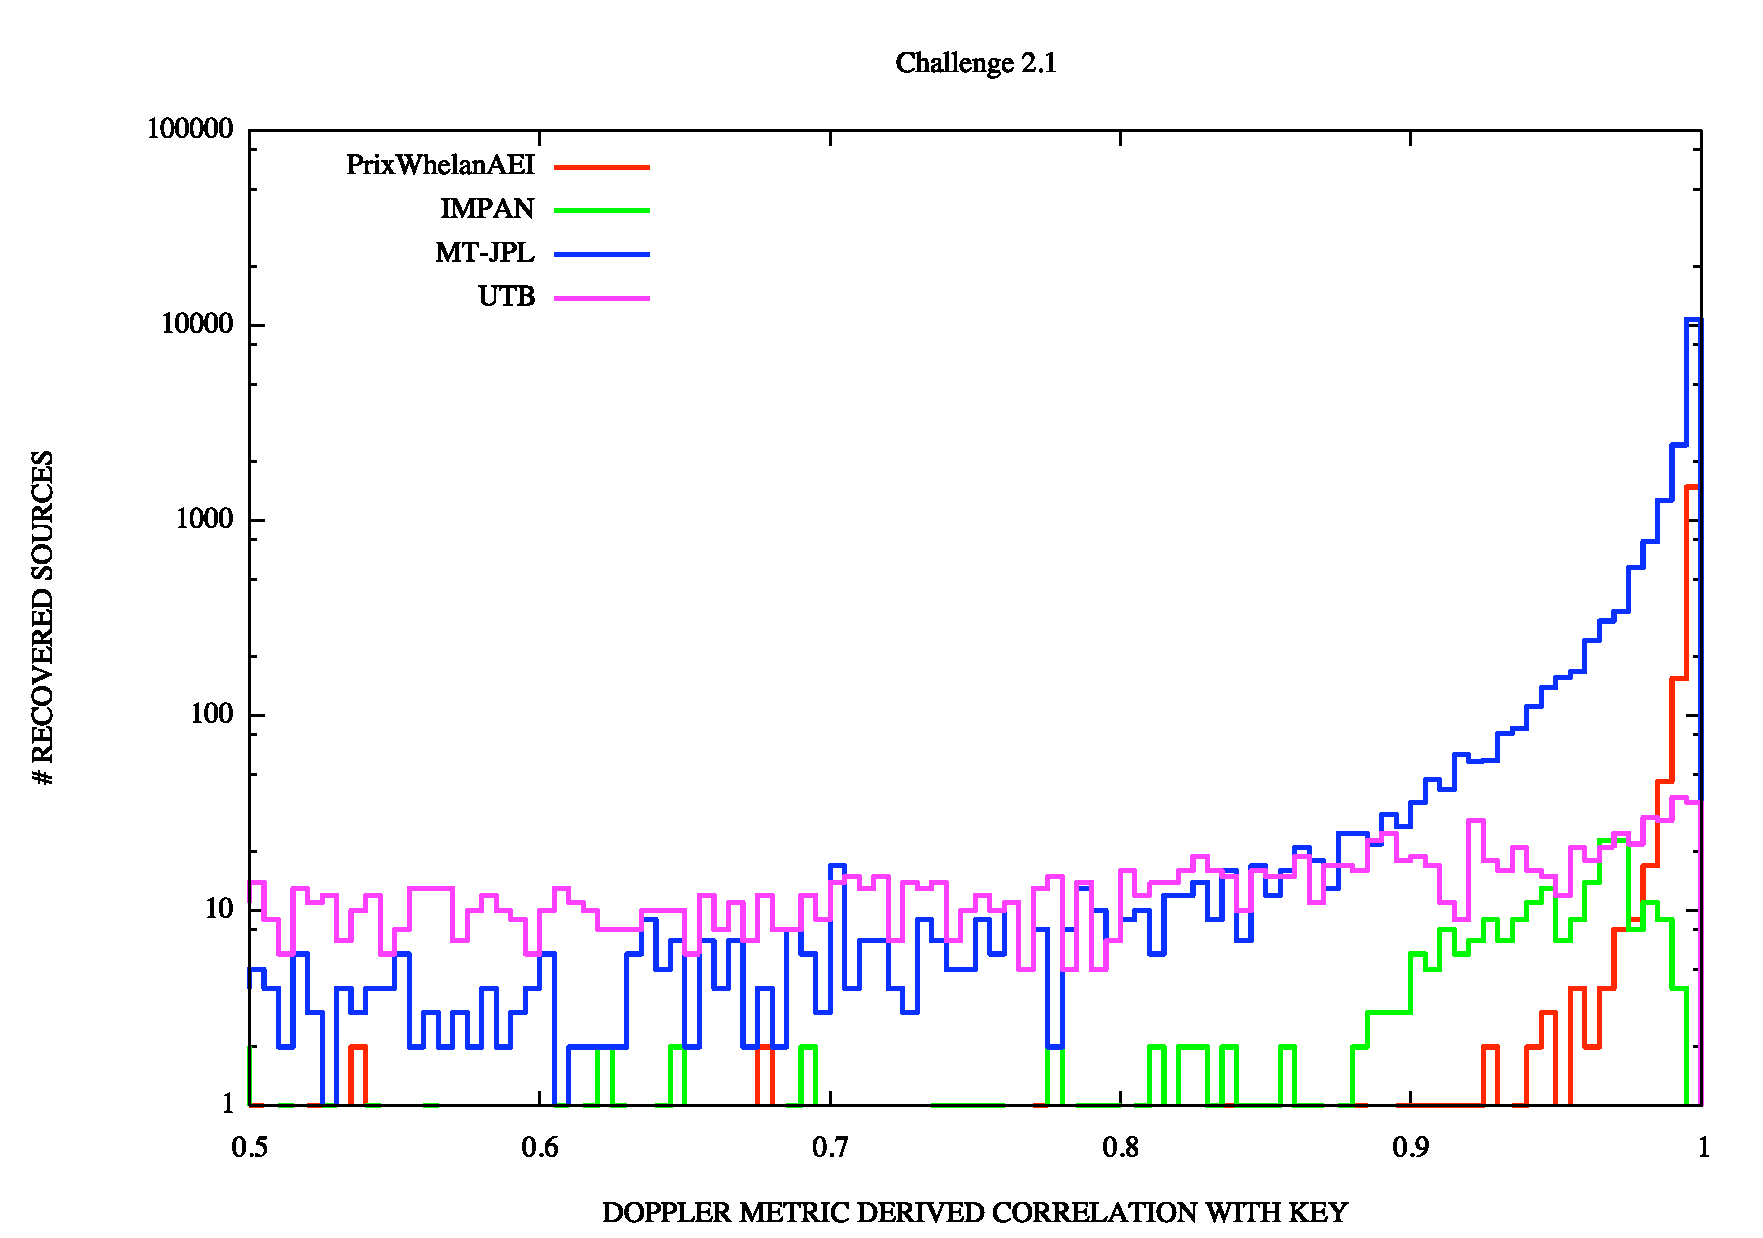
\includegraphics[width=0.5\textwidth]{dcorrelation}
\caption{XXX\label{fig:correlation}}
\end{figure}

One way to proceed is to associate the reported and true sources that have the strongest signal correlation (limiting the search to the ``bright'' $\mathrm{SNR} > 2$ true sources that could in principle have been found) [[can true sources be ``reused'' in this association?]]: in the left panel of figure \ref{fig:correlation} we show the distribution of correlations generated in this process for data set 2.1. Another way is to associate reported and true sources that minimize the \emph{Doppler metric} that spans the frequency--sky-location subspace of the full parameter space, and automatically maximizes correlation over the \emph{extrinsic parameters} (amplitude, polarization, inclination, initial phase): the right panel of figure \ref{fig:correlation} shows the resulting distribution of correlations. The UTB entry, which includes frequency and sky position but not the extrinsic parameters, can only be plotted this way. Generally, this is a softer criterion, and all searches do better (especially the PrixWhelanAEI entry, whose long-wavelength approximation for the LISA response is prone to extrinsic-parameter errors).
%
\begin{figure}
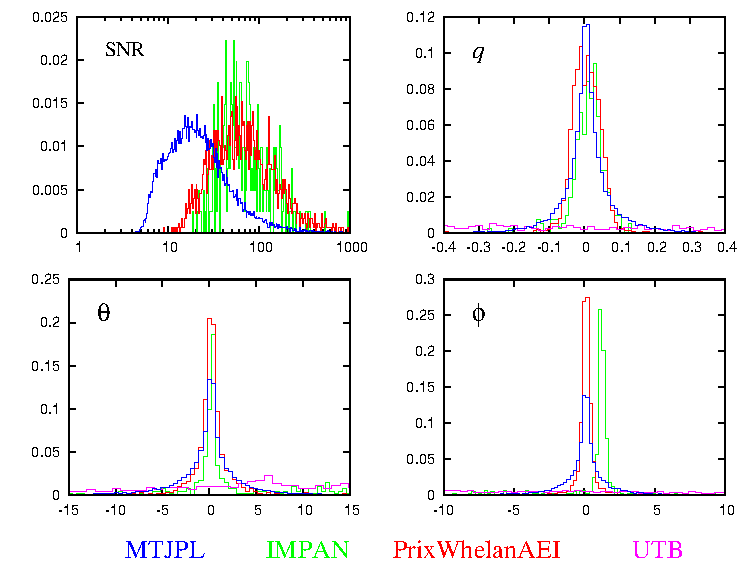
\includegraphics[width=0.5\textwidth]{intrinsic}
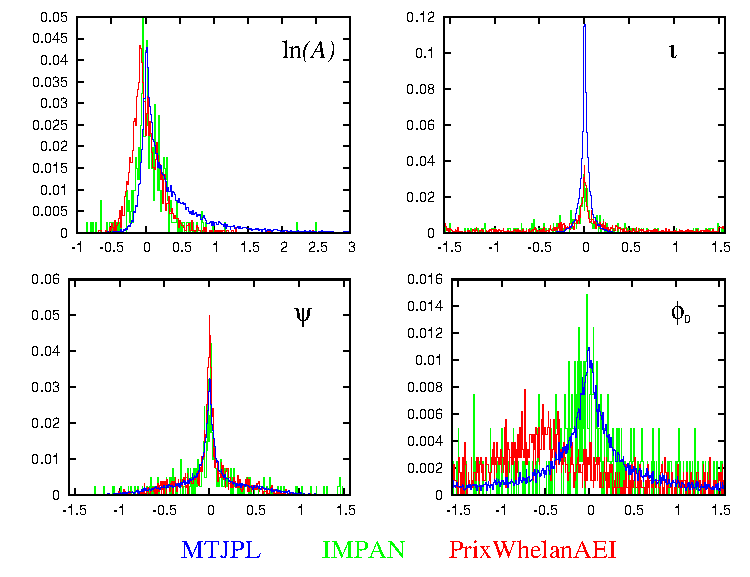
\includegraphics[width=0.5\textwidth]{extrinsic}
\caption{XXX\label{fig:paramerrors}}
\end{figure}

Figure \ref{fig:paramerrors} shows the SNRs of the recovered sources and the errors for the intrinsic and extrinsic parameters, computed after associating sources by correlation (and by Doppler metric only for the UTB entry), again for data set 2.1. The error in frequency is in most cases within a small fraction of a Fourier bin; the errors in sky position are within a few degrees; by contrast the errors in the amplitude and in the (extrinsic) orientation angles are larger. The $\phi_0$ graph for the PrixWhelanAEI suggests a systematic error in the definition of initial phase. [[Was there some correspondence about this?]]

These challenges demonstrated a solid capability in analyzing signals from the Galaxy and resolving a large number of binaries. At the same time, they emphasized the difficulty of determining when a source is resolvable, and of defining (at least operationally) a notion of \emph{identity} for recovered sources. These problems deserve careful, targeted work.

\section{Data set 2.2: MBH binaries (over the Galaxy)}

Four groups reported parameters for the MBH binaries in the 2.2 data set:
\begin{description} 
\item[AEIse.] Babak and Porter used $\mathcal{F}$-statistic, template-bank--based matched filtering, followed by an MCMC stage;
\item[MTAEI.] Cornish and Porter used MCMC matched filtering in a \emph{frequency-annealed} scheme where shorter, lower-frequency templates are used in the initial phases of the search and progressively extended;
\item[JPLCT.] the JPL--CIT collaboration used a three-stage pipeline consisting of a track search in the time--frequency (TF) plane, followed by template-bank--based matched filtering, and by an MCMC refinement;
\item[LisaFrance.] the French collaboration used a TF track search alone, and therefore reported only mass and time-of-coalescence parameters.
\end{description}
All the four MBH binaries in the data set (MBH-1, 2, 4 and 5, with total SNRs $\sim$ 2583, 25, 174 and 117) were positively detected by AEIse, MTAEI, and JPLCT; the TF method used by LisaFrance identified MBH-1 and 4, but not MBH-2, and could report only a time of coalescence for MBH-5.
%
\begin{table}
MBH-1. First line: true parameters and SNR. Then parameter errors and recovered SNR.
\caption{\label{tab:mbh1}}
\end{table}
%
\begin{table}
MBH-4. As above, but give also the relative odds reported by the collaborations for the multiple candidates.
\caption{\label{tab:mbh4}}
\end{table}

Tables \ref{tab:mbh1} and \ref{tab:mbh4} show fractional parameter errors for MBH-1 and 4 (complete results can be found at the URL XXX), together with the SNR recovered by the best-fit candidate of each group, computed as 
%
\begin{equation}
\mathrm{SNR}_\mathrm{best}  = \frac{(A_{true}|A_{best}) + (E_{true}|E_{best})}
{\sqrt{(A_{best}|A_{best}) + (E_{best}|E_{best})}},
\end{equation}
%
with $(\cdot|\cdot)$ the usual noise-weighted inner product, and $A = (2X - Y - Z)/3$ and $E = (Z-Y)/\sqrt{3}$ two noise-orthogonal TDI observables (see, e.g., VCT). In table \ref{tab:mbh1}, we see that compared to MTAEI, the JPLCT search for MBH-1 locked onto a secondary probability maximum with only slightly lower $\mathrm{SNR}_\mathrm{best}$, but with sky positions off by several degrees, which also led to errors in the other parameters. MBH-4 (table \ref{tab:mbh1}) is an interesting example of a true (at least) bimodal probability distribution. MTAEI and JPLCT reported two candidates at rather different sky locations, with relative probability ratios of 1:1 and 1.18:1, respectively. The position and orientation of this source relative to LISA, which resulted in a very weak signal in one of the noise-orthogonal observables, probably concurred in degrading LISA's sensitivity to sky position.

This challenge demonstrated a solid capability in the detection and parameter estimation of MBH inspirals of moderate SNR over a strong Galactic background, at least if the inspirals are close to our idealized model: circular and adiabatic, with negligible spin effects. These restrictions are being relaxed for the upcoming Challenge 3.

\section{Data sets 1.3.X: EMRIs}

[[Develop this in analogy to the MBH section.]]

\begin{description}
\item[BBGP] Babak/Barack/Gair/Porter (time-annealed MCMC)
\item[MT] Cornish (segmented MCMC)
\item[EtfAG] Gair/Mandel/Wen (TF track search)
\end{description}

\section{Conclusion}

We're happy:
\begin{itemize}
\item Participation is strong (but we need more, try 1B!)
\item A lot of work is being accomplished
\item Results are comforting
\item We’re showing that LISA data analysis is possible
\item Difficulty is incremental, but no big issues of principle are foreseen
\item The MLDC infrastructure (LISAtools) can be used for many other experiments outside the mainline challenges
\end{itemize}

Resources:
\begin{itemize}
\item MLDC official site:	\url{astrogravs.nasa.gov/docs/mldc}
\item MLDC taskforce wiki: \url{www.tapir.caltech.edu/dokuwiki/listwg1b:home}
\item Mailing lists: \url{lisatools-mldc@gravity.psu.edu} (formulation) \url{lisatools-challenge@gravity.psu.edu} (participants)
\item LISAtools software (including full MLDC pipeline): \url{lisatools.googlecode.com}
\end{itemize}

% [[After submitting this, we should put evaluation documents on the tapir mldc webpage.]]

\ack

This work was carried out at the Jet Propulsion Laboratory, California Institute of Technology, under contract with the National Aeronautics and Space Administration. MV was supported by LISA Mission Science Office and by JPL's Human Resources Development Fund.

% \appendix

% \section{SNR and cross-spectra}

\section*{References}

\begin{thebibliography}{99}
%
\bibitem{lisa} Bender P, Danzmann P and
  the LISA Study Team 1998 ``Laser Interferometer Space Antenna for the Detection of Gravitational Waves, Pre-Phase A Report'' \textbf{MPQ 233} (Garching: Max-Planck-Instit\"ut f\"ur
  Quantenoptik) 
%
\bibitem{JKS98}
P.\ Jaranowski, A.\ Kr\'olak, and B.\ F.\ Schutz, Phys.\ Rev.\ D
{\textbf 58}, 063001 (1998).
%
\bibitem{KTV04} A. Kr\'olak, M. Tinto, and M. Vallisneri, {\it Phys. Rev. D}, {\bf 70},
022003 (2004).
%
\end{thebibliography}

\end{document}




